% !TEX root = /Users/zhuzhuangdi/Desktop/MSUCourses/MachineLearning847/17spr_wang_zhu_du/Final/final_report.tex
\section{Evalutaion}
For each of the three approaches, we use the same preprocessing steps to get the same features. Then we compare among the  Song Ci generated from the three approaches based on three metrics : structure, rhyme, and semantics. 
% !TEX root = /Users/zhuzhuangdi/Desktop/MSUCourses/MachineLearning847/17Project/17spr_wang_zhu_du/Middle/middle_report.tex
\section{Data Description}   
For our experiment, we obtained dataset for both Tang Shi and Song Ci. Many research were conducted for automatically generating Tang Shi. So we can evaluate our experiment result by comparing with these machine-created Tang Shi. And then we can move forward to Song Ci.
\subsubsection{Tang Poetry Corpus}
We use Quan Tangshi as our Tang Poetry corpus.\cite{1960quantangshi}. It was commissioned by Yin Cao in 1705 and published under the name of Kangxi Emperor. It contains 49,000 lyric poems (in the dataset we used it has 49,274 poems) and is believed the largest collection of Tang poetry. We obtained the dataset from the server of \cite{zhang2014chinese}.
\subsubsection{Song Ci Corpus}
\subsubsection{Background Survey}
% For this initial step, we plan to search for related works to computational literary creation to gain the basic knowledge of Song Ci.
%
We conducted large amount of survey on the state of the art approaches of SongCi generation.
%
We find that this task attracts many interests both from the Natural Language Processing area and Machine Learning area.
%
The approaches can be generalized into two kinds:  We either specify the generation rules (using templates), or build a model which can learn these rules automatically ( using neural network).
%
We also implemented some of the approaches proposed in previous work.
%
%
%
\subsubsection {Corpus Search and Analysis}
%
The dataset we use contains 18668 Ci, which contains a total number of 1183 poets and 1170 Pai. This dataset basically covers Ci generated during the entire Song Dynasty and the beginning of Yuan Dynasty. We analyze the number of poems wrote by each poet, which shown in Figure \ref{fig:poet}. Most of the poems are created by the first poets. The one that creates the most poems is Qiji Xin, one of the most famous poet of the Southern Song Dynasty. His poems covers a wide range of styles. Among all those poems, the bold style is most will known by now. In addition, we statistic the Pai of each poem. Ci was first used as a lyric, and Pai is the name of the tune. Each Pai has a specific melody and rhythm, so Ci has a fixed format requirements, such as the number of sentences, the number of words per sentence, pronunciation of those words, rhyme and so on. The statistical result is shown in Figure \ref{fig:Pai}. The most popular Pai is Silk-Washing Stream, followed by Prelude To Water Melody, Partridge Sky, Pusaman and River of Red. And there is good reason to believe that the songs that corresponding to these Pai are beautiful in melody, lively in rhythm and easy to sung, which caused them to be so popular in ancient China.
\begin{figure}[htbp]
	\centering
	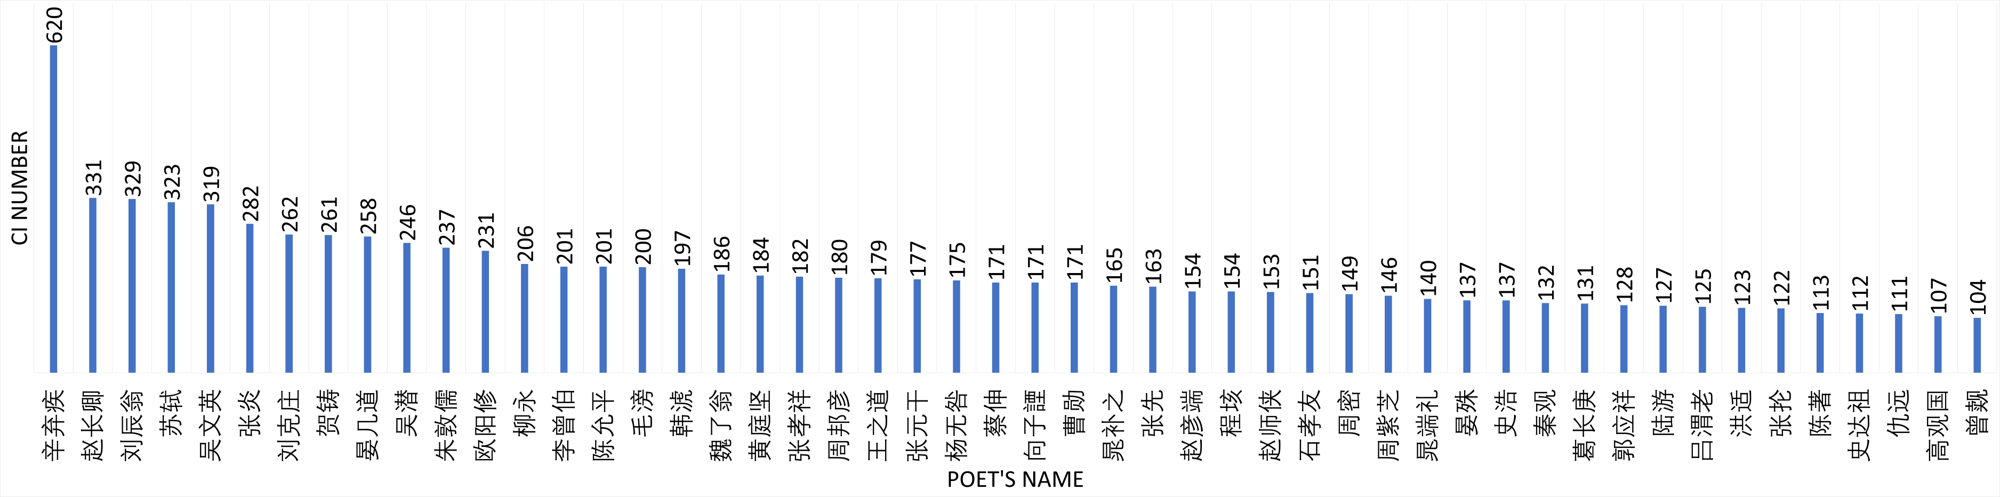
\includegraphics[width=0.9\linewidth]{poets.png}
	\caption{Poem Number Created by Top 50 Productive Poets}
	\label{fig:poet}
\end{figure}

\begin{figure}[htbp]
	\centering
	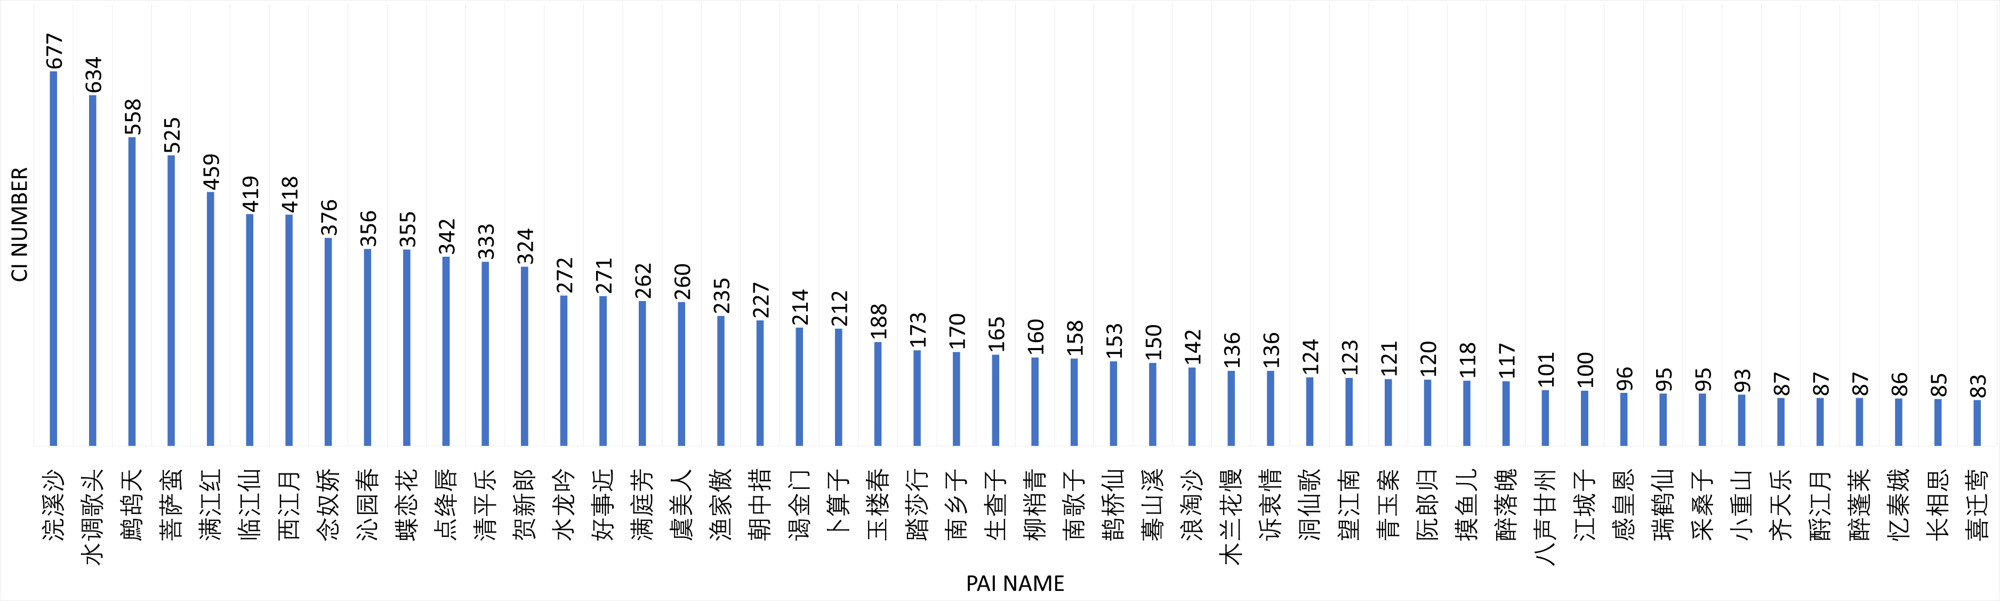
\includegraphics[width=0.9\linewidth]{Pai.png}
	\caption{Poem Number of Top 50 Popular Pai}
	\label{fig:pai}
\end{figure}
%

Word frequency analysis is to statistic and analyze the number of important words in the text, which is an important method of text mining. It is a traditional and useful content analysis method. The basic principle is to determine the overall style and theme of the entire article by the frequency of the words. By analyzing the word frequency in the poems, we have a general understanding of the style of poems and the process of writing those the poem, which can help us get more familiar with the grammar rules and themes of Ci. The most commonly used words can reveal common theme of Ci and the corresponding feelings. For example, we analyzed word frequency of season in our database. The result is shown in Figure \ref{fig:season}. We found that spring related words reached 2606, these words appeared in our dataset for 9210 times. Followed by autumn, there are 1167 words associated with autumn and appeared 3992 times. The unique scene in spring and autumn can trigger people's emotions, which might be the reason that so many poems are related with these two seasons.
\begin{figure}[htbp]
	\centering
	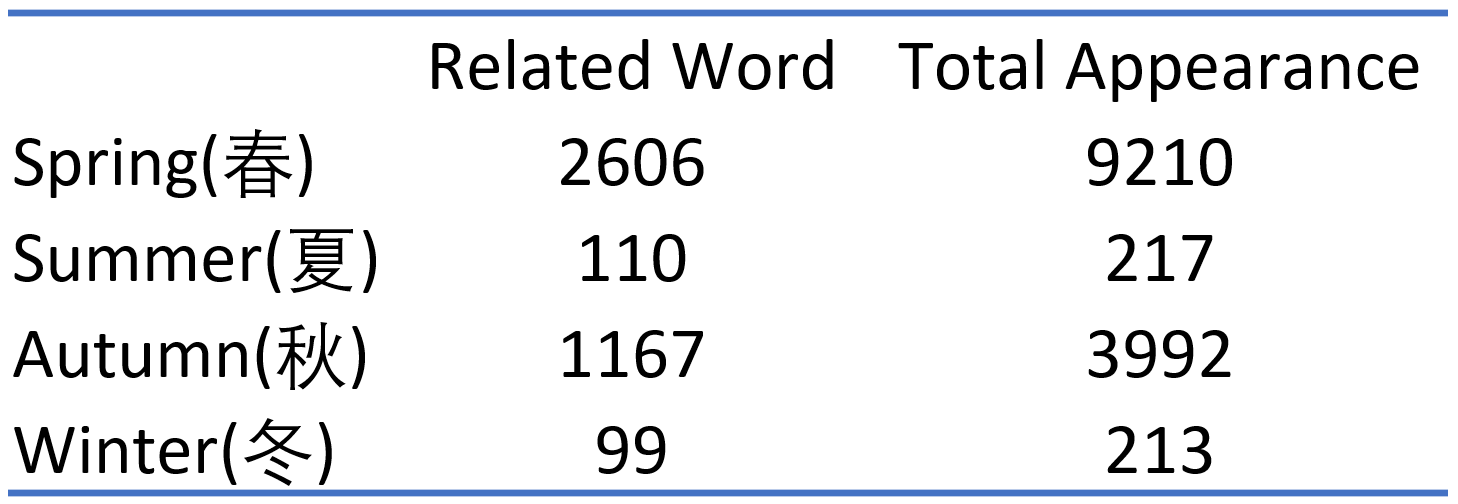
\includegraphics[width=0.8\linewidth]{season.png}
	\caption{Statistical Data of Season Related Word Frequency in Dataset}
	\label{fig:season}
\end{figure}
%
From most frequently used words, shown in Figure \ref{fig:wordcloud}, we found that the moon, east wind, mortal world, wine, dream, rain, flowers , sunset, old friends are the most commonly used images. Commonly used places, including Jiangnan, West Lake, Changan, Fairy Isle, Yangzhou. Commonly used verbs including laugh , come back, go back, lovesickness, look back, meet by chance. Commonly used emotions are hate, worry, hard, sigh, desolate, haggard. These words represent a very broad theme and style of Ci, including the description of leaving and missing, pride and enthusiasm, seasonal terms, chanting things, chanting nostalgia and so on.
%
\subsubsection{Implementation of Genetic Algorithm and Additional Information Collection}
Initially, we collect additional information about syntactic pattern of sentences with different length, format of tone pattern and rhythm and format of different Cipai from past research work on Song Ci.
%
The syntactic pattern for traditional Chinese poem are shown in Figure \ref{fig:syntactic}.
%
In this figure, sentence length means how many characters are in this sentence.
%
'*' in syntactic pattern represent a character and '/' used to split sentences into several parts.
%
Words in these sentence shell not cross the split.
%
Otherwise, this sentence may not be that easy to read and understand.
%
What we can see is that one several different syntactic patterns are allowed for the same sentence length, such as sentence with five characters, the sentence can either have two characters at the beginning then three characters or vice versa.
%
This actually gives traditional poems much freedom on expression.

\begin{figure}[htbp]
	\centering
	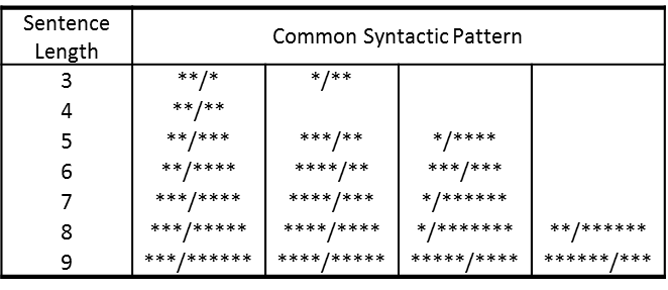
\includegraphics[width=0.9\linewidth]{syntactic.png}
	\caption{Syntactic Patterns for Sentences with Different Length.}
	\label{fig:syntactic}
\end{figure}

Then we defined several properties for characters and words in Song Ci.
%
Tone pattern which is called pingze in Chinese, we use 1 to represent Ping, 2 to represent Ze.
%
There are twenty four rhythm in Chinese, in traditional Chinese poem, usually the last characters of every sentence are required to be the same rhythm.
%
 We get pingze and rhythm information from existing datasets.
%
The correlation between words we use python package word2vec(https://code.google.com/archive/p/word2vec/) to quantify the relationship between words, which will be later used in generating Song Ci that is closely related with keywords.


We also extract format for different Cipai from existing dataset, which contains sentence number, length, tone pattern and the delimiter of each sentence.
%
For example, Huanxisha is a very popular Cipai in Song Ci.
%
The sentence format of Huanxisha is ['0201021', '0102211', '0102211', '0201122', '0102211', '0102211'].
%
In this format, there are 6 sentences, each sentence contains 7 characters.
%
0,1 and 2 represent the requirement of Pingze, 0 means both ping and ze will work in this position.
%
Each sentence will apply the syntactic pattern previous defined.


\begin{figure}[htbp]
	\centering
	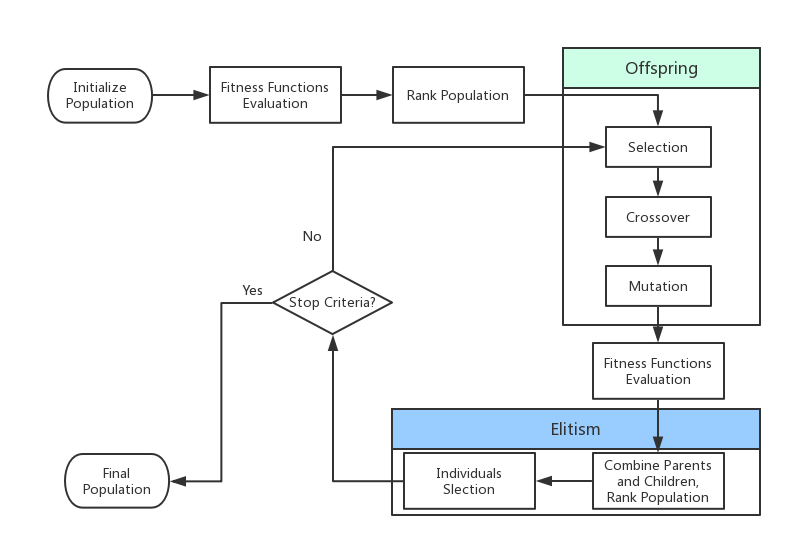
\includegraphics[width=0.9\linewidth]{GA.png}
	\caption{Process of Generating Song Ci by Genetic Algorithm}
	\label{fig:GA}
\end{figure}


Based on the rule of compose Song Ci, we found that Song Ci is a combination of words.
%
Thus, traditional method with pre-defined rules can easily generate Song Ci with correct format.
%
For genetic algorithm, we use a Cipai title and several keywords as input.
%
Based on the sentence format and tone requirement, words that are highly correlated with keywords are selected as candidate words for initial population.
%
Based on randomly chosen rhythm, pre-defined sentence form, syntactic patterns and tone patterns, program randomly put words that satisfied all the requirement to each position and generate the first generation of candidate poems.
%
The initial population is strictly follows the format and rules of Song Ci.


Then all candidate poems go through the fitness evaluation process.
%
Based on score of syntactic and semantic correctness, correlation with keywords, correlation between sentences and tone, rhythm pattern, a fitness value is generated for each candidate poem.
%
Best several individuals are selected as parents to generate offspring with mutation and crossover.
%
Mutation means characters within this poem will change randomly.
%
Crossover represents two poems randomly exchange part of their sentences and form two new poems.
%
All offspring and parents together forms the next generation and need to be evaluate on fitness value.
%
Then this iteration will continue until satisfactory fitness level has been reached or a maximum number of generations has been produced.


In the last, we'll manually choose best poem from the final generation.
%
The whole process is shown in Figure \ref{fig:GA}.
%
Final results are shown in following section.


\subsubsection{ Implementation of a Vector Space Model }
Vector space models (VSMs) represent words in a continuous vector space where semantically similar words are mapped to nearby points.
%
We implemented this model to find the semantic relations between each Chinese character, so that given a few of keyword characters, such as 'spring' and 'beauty', we can generate poetries with coherent meanings using characters which are close to these keywords in the vector space.
%
%We use a predictive method to implement this  model based on the TensorFlow programming package \cite{tensorflow}.
%
We give a visualized result in Figure \ref{fig:VSM}. The figure is embeded with 100 Chinese characters in a 2-D space, which are randomly chosen from the most frequent 500 Chinese characters in the Song Ci corpus. The 2-D space corresponds to the first two dimensions in the vector space. We can see that words such as `spring', `sunny', and `breeze' are very close in the 2-D space, which convey similar sentimental feelings to readers.



\begin{figure}[htbp]
	\centering
	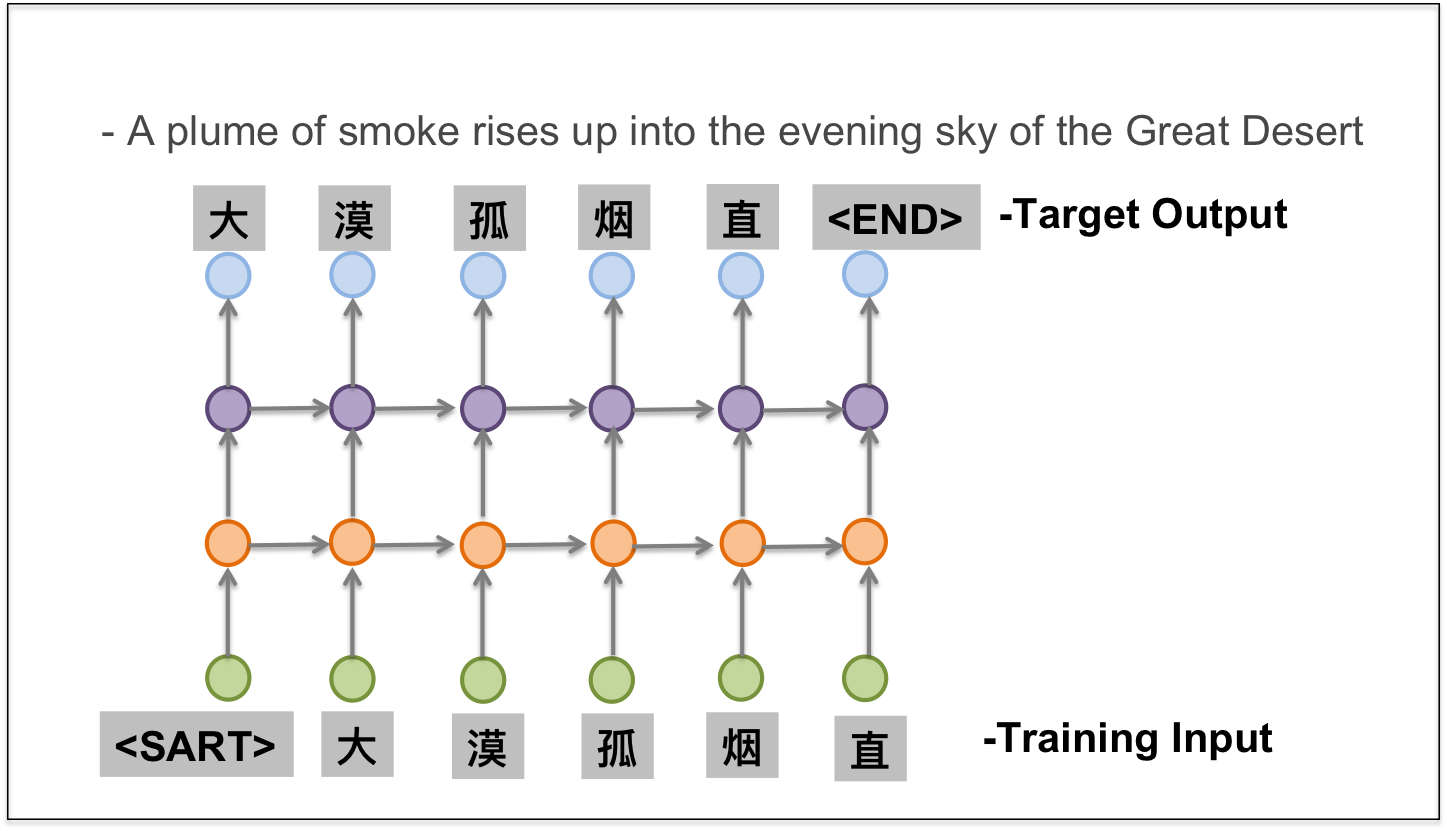
\includegraphics[width=0.9\linewidth]{RNN_model}
	\caption{Workflow of the RNN model}
	\label{fig:rnn_workflow}
\end{figure}

\begin{figure}[htbp]
	\centering
	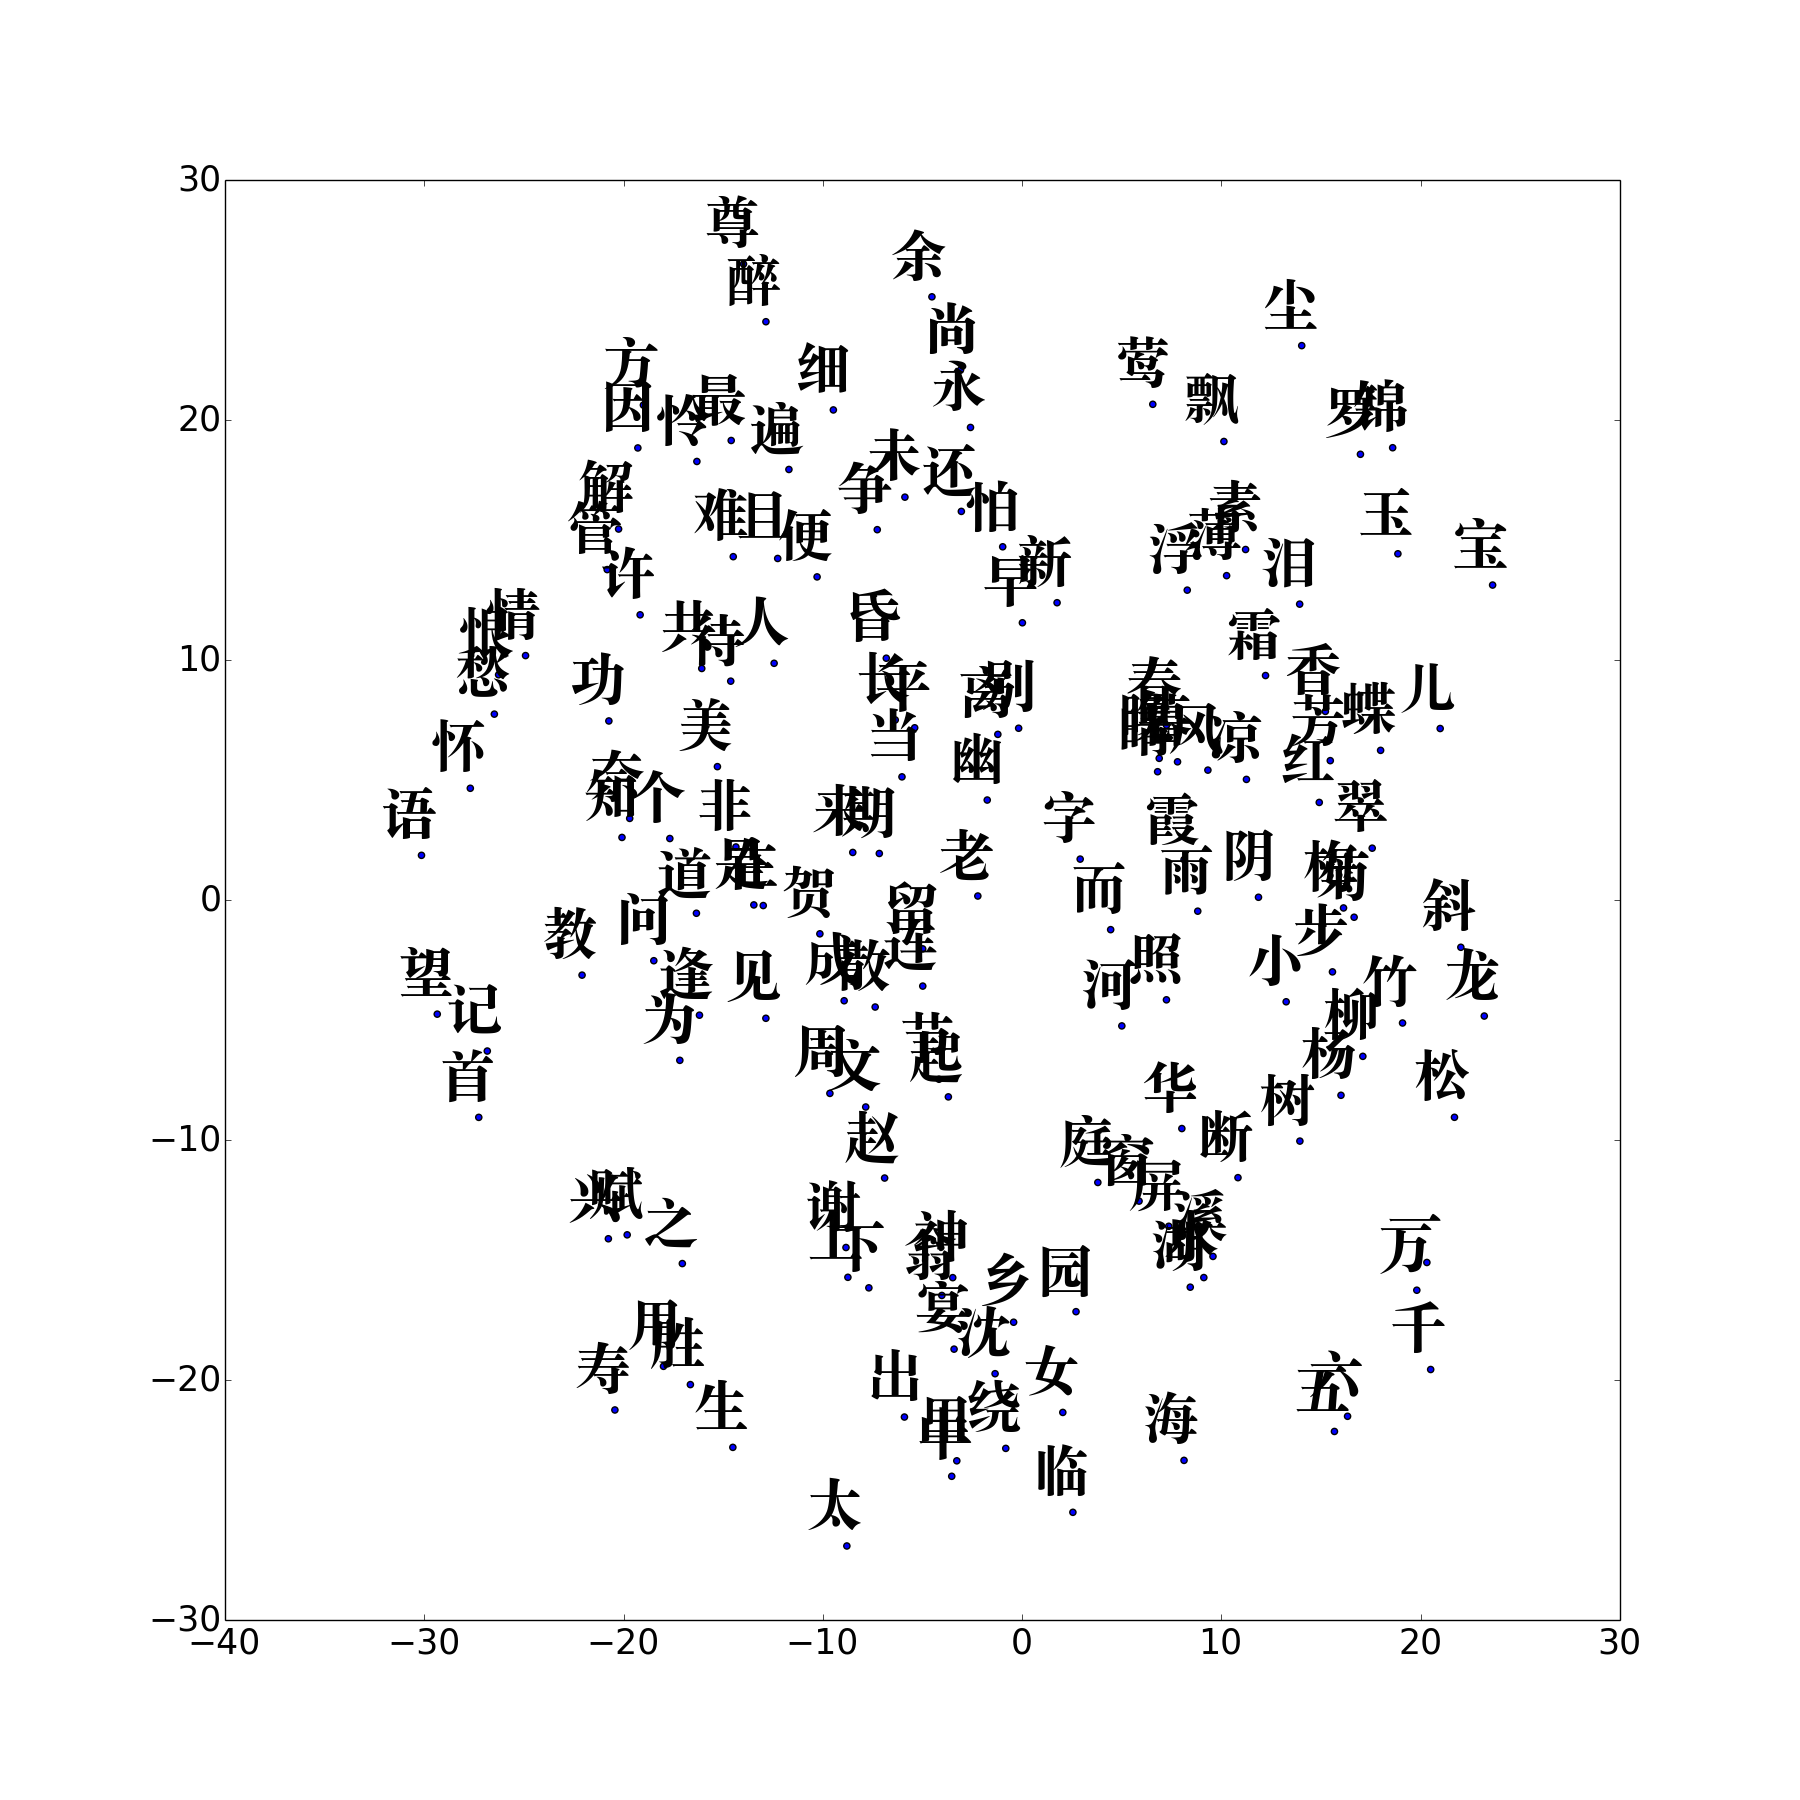
\includegraphics[width=0.9\linewidth]{tsne.png}
	\caption{Projections of most frequent characters to a 2-D space using the word embedding model}
	\label{fig:VSM}
\end{figure}



\subsubsection{Implementation of RNN Model} 
%
We used deep learning Python modules called \emph{TensorFlow} \cite{tensorflow} to implement our RNN model. 
%
We present a preliminary result in Figure \ref{fig:poetry}, which is a quatrain poem.
\begin{figure*}[htbp]
	\centering
	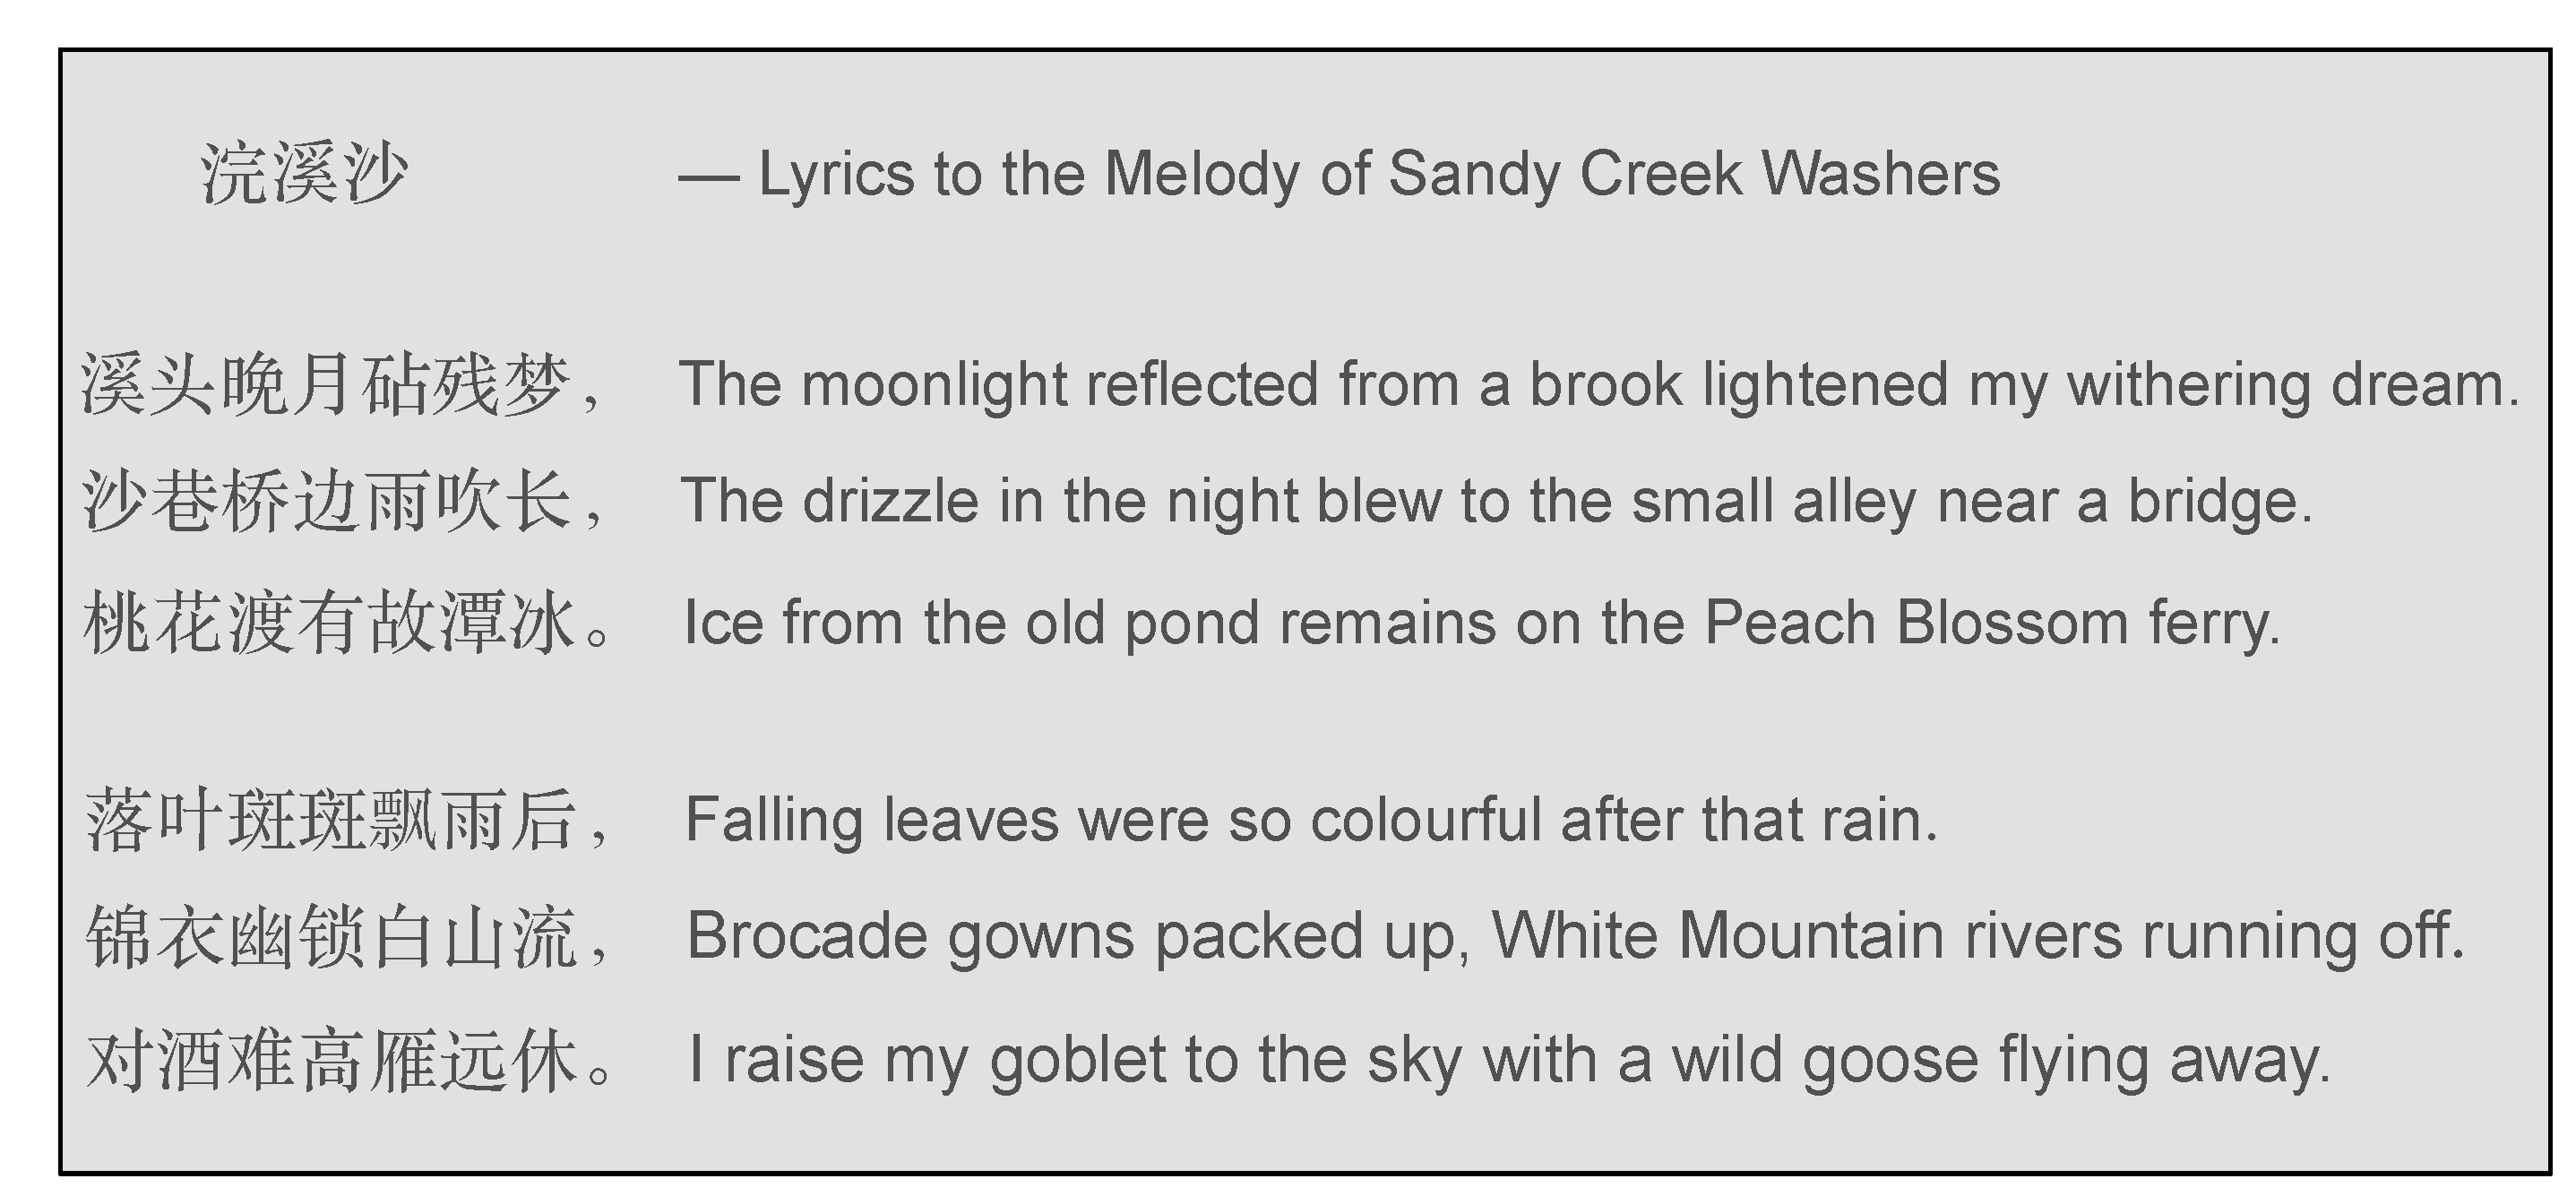
\includegraphics[width=0.8\linewidth]{poem_template}
	\caption{A Song Ci generated using LSTM}
	\label{fig:poetry}
\end{figure*}

\begin{figure*}[htbp]
	\centering
	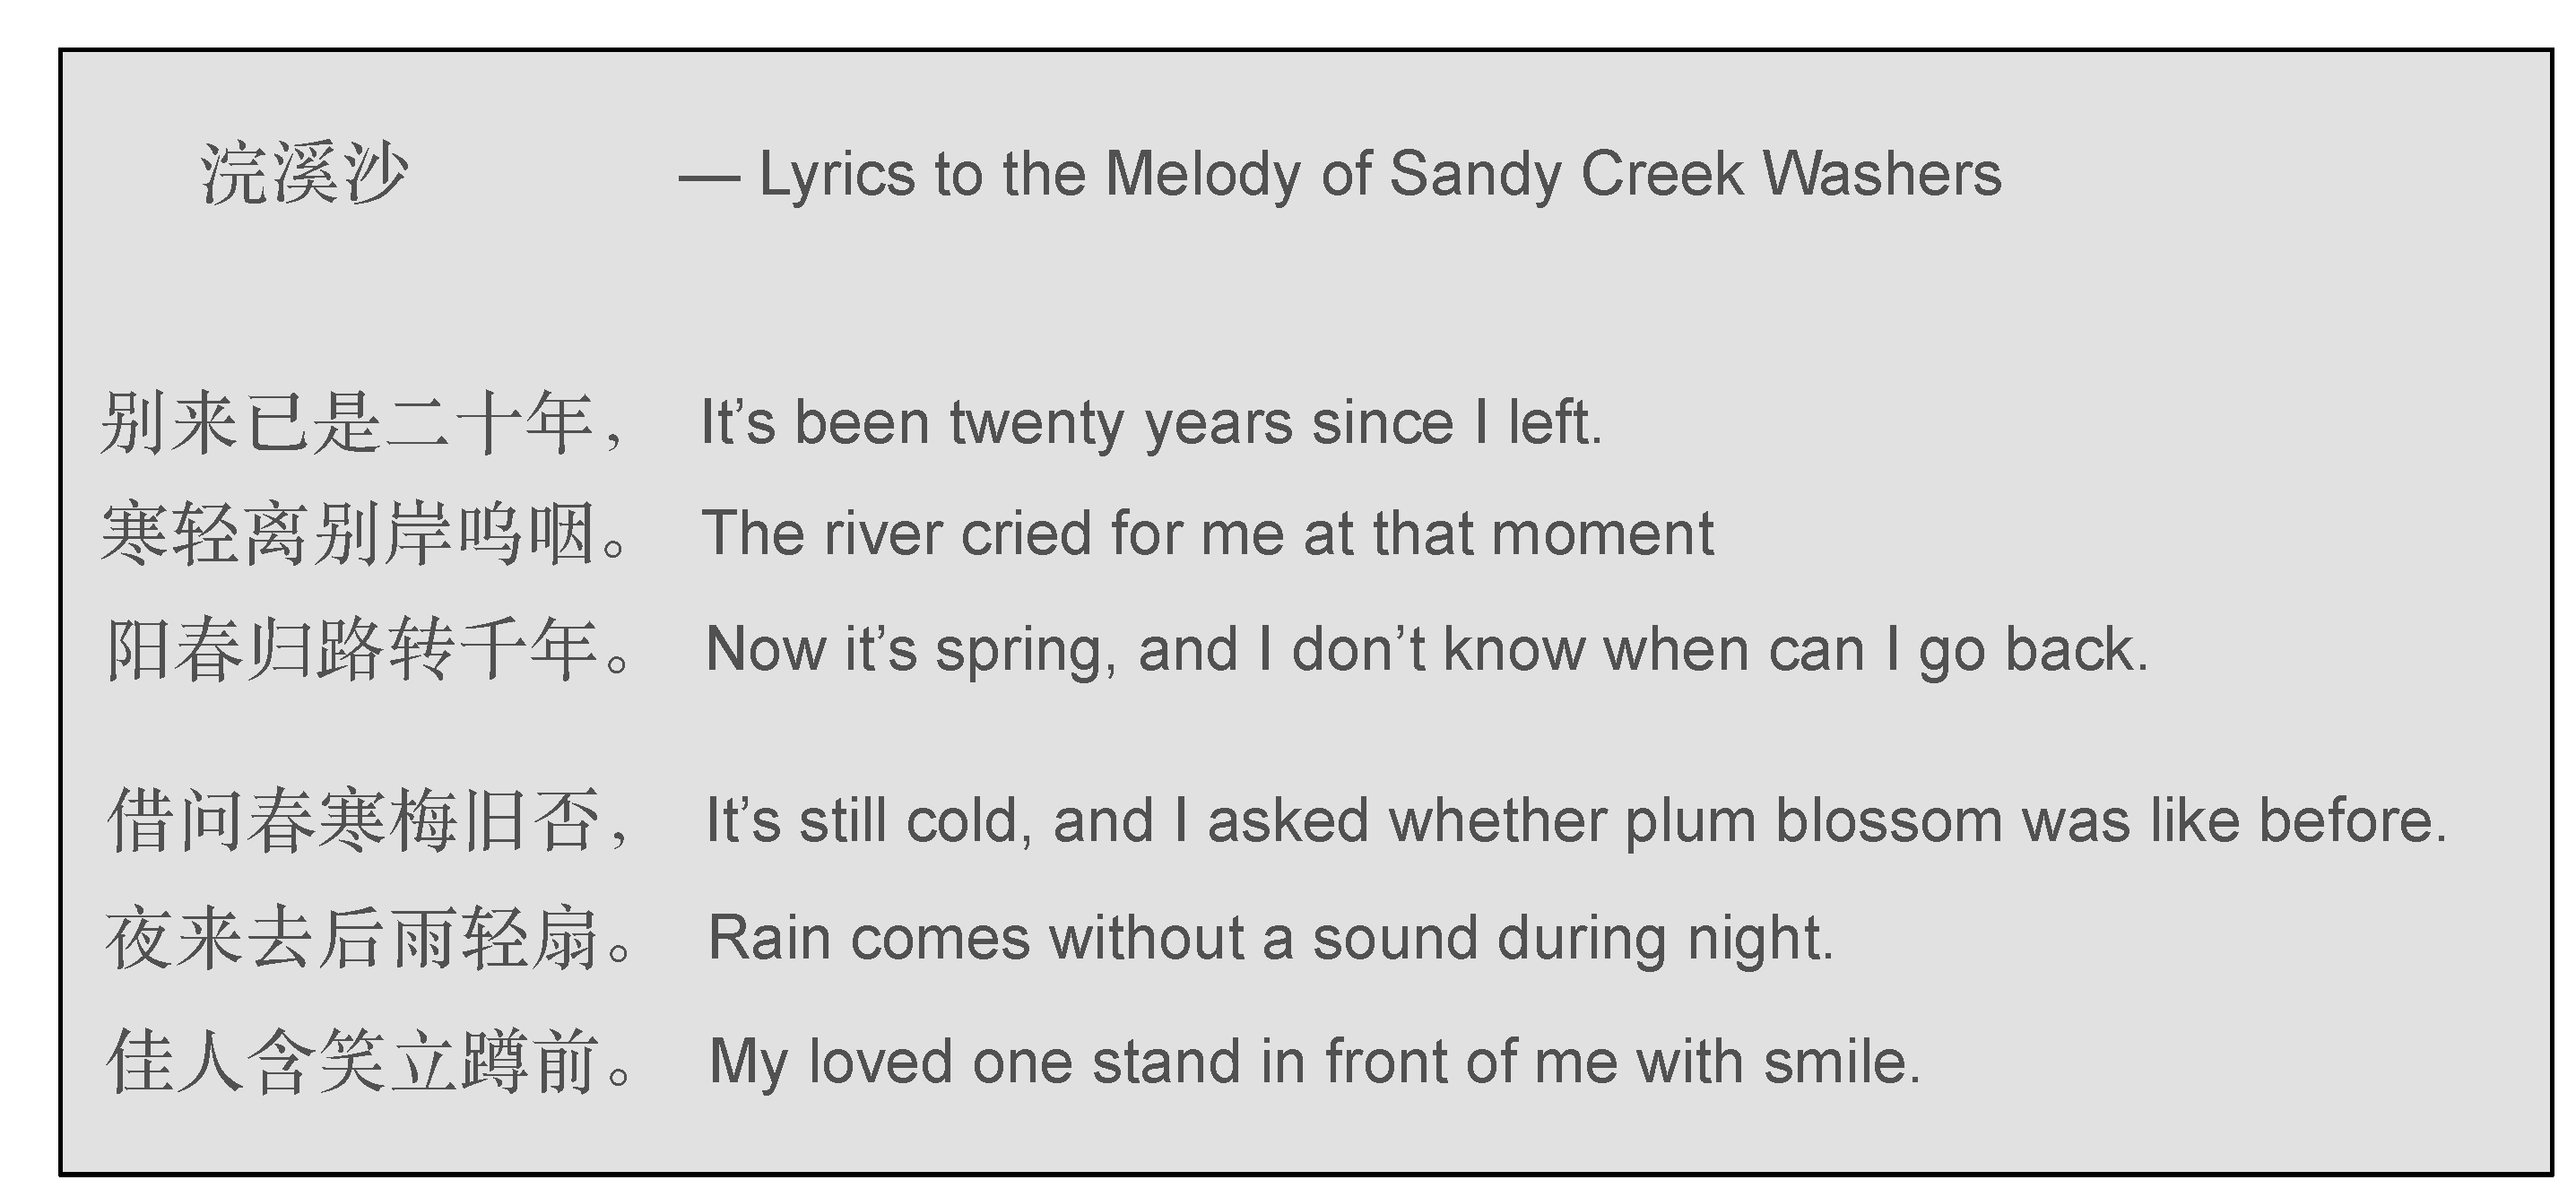
\includegraphics[width=0.8\linewidth]{poem_template2}
	\caption{A Song Ci generated using Genetic Algorithm }
	\label{fig:poetry}
\end{figure*}
